
\section{Algorithm} \label{sec:algorithm}

As a means of producing fewer energy violations when scheduling system tasks, We have developed a technique for reducing energy violations when scheduling tasks, called the \emph{Smooth to Average Method} (\textsc{STAM}). This heuristic takes into account the average energy requirements per unit time of all tasks in a given task list. We generate a set of equivalent virtual tasks by increasing the duration of any task that uses greater than average energy per unit time until its energy used per unit time is near the average. In these virtual tasks, the total energy remains the same as for real tasks' energy but it is spread over a longer duration.  Virtual tasks cannot be scheduled to run at the same time.  Once the virtual tasks are scheduled, the real tasks are inserted at the end of the corresponding virtual task's timeslot.  Thus a real task that consumes high energy is guaranteed to run after an idle period, reducing the likelihood that the system will run out of energy when the task runs.

\begin{algorithm}[htb]
\label{stamalg}
\begin{algorithmic}
\STATE INPUT: $realTasks$ \COMMENT {list of [period, duration, energy]} 
\STATE INPUT: $N$ \COMMENT {number of tasks}
\STATE OUTPUT: $vTasks$ \COMMENT {same format as $realTasks$}
\STATE $meanEnergy \gets mean(realTasks[:,3])$
\FOR{$i = 1$ \TO $N$}
\IF{$taskList[i,3] > meanEnergy$}
\STATE $taskEnergy \gets realTasks[i, 2] * realTasks[i,3]$
\STATE $vDuration \gets \lceil \frac{taskEnergy}{meanEnergy} \rceil$
\STATE $vEnergy \gets \frac{taskEnergy}{vDuration}$
\STATE $vTasks[i,:] \gets [taskList[i,1]~~vDuration~~vEnergy]$
\ELSE
\STATE $vTasks[i,:] \gets taskList[i,:]$
\ENDIF
\ENDFOR
\end{algorithmic}
\caption{Generate \textsc{STAM} Task List}
\end{algorithm}

The \textsc{STAM} algorithm calculates the energy consumption of each task by multiplying its runtime by the task's energy consumption per time unit. After taking the mean energy consumption across all of the tasks in the task list, each task is compared to the this value and virtual tasks are generated accordingly. If the given task's energy consumption is above the mean energy value, the virtual duration is calculated by taking the ceiling of the energy area of the task divided by the calculated energy mean. This will extend the duration of the virtual task allowing the total energy consumed to be more evenly distributed across the duration of the task's runtime. If the given task's energy consumption is below the calculated energy mean, the algorithm is unable to perform any smoothing and  will use the unchanged physical task to generate a schedule.
\begin{figure}[htb]
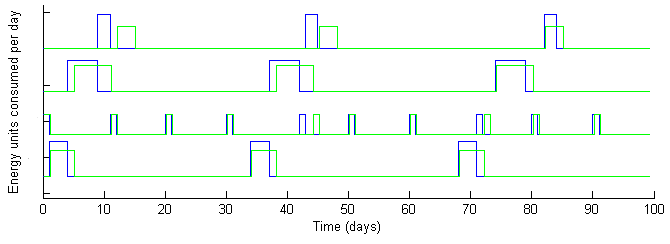
\includegraphics[scale=0.38]{stamtasks.png}
\caption{EDF schedules for four tasks and their STAM equivalents}
\label{fig:stamtaskplot}
\end{figure}

Figure~\ref{fig:stamtaskplot} shows 